\documentclass[a4paper, 12pt]{article}

%%% Работа с русским языком
\usepackage{cmap}					% поиск в PDF
\usepackage{mathtext} 				% русские буквы в формулах
\usepackage[T2A]{fontenc}			% кодировка
\usepackage[utf8]{inputenc}			% кодировка исходного текста
\usepackage[russian]{babel}	% локализация и переносы

%%% Дополнительная работа с математикой
\usepackage{amsmath,amsfonts,amssymb,amsthm,mathtools} % AMS
\usepackage{icomma} % "Умная" запятая: $0,2$ --- число, $0, 2$ --- перечисление

%% Номера формул
%\mathtoolsset{showonlyrefs=true} % Показывать номера только у тех формул, на которые есть \eqref{} в тексте.

%% Шрифты
\usepackage{euscript}	 % Шрифт Евклид
\usepackage{mathrsfs} % Красивый матшрифт

%% Поля
\usepackage[left=2cm,right=2cm,top=2cm,bottom=2cm,bindingoffset=0cm]{geometry}

%% Русские списки
\usepackage{enumitem}
\makeatletter
\AddEnumerateCounter{\asbuk}{\russian@alph}{щ}
\makeatother

%%% Работа с картинками
\usepackage{graphicx}  % Для вставки рисунков
\graphicspath{{images/}{images2/}}  % папки с картинками
\setlength\fboxsep{3pt} % Отступ рамки \fbox{} от рисунка
\setlength\fboxrule{1pt} % Толщина линий рамки \fbox{}
\usepackage{wrapfig} % Обтекание рисунков и таблиц текстом

%%% Работа с таблицами
\usepackage{array,tabularx,tabulary,booktabs} % Дополнительная работа с таблицами
\usepackage{longtable}  % Длинные таблицы
\usepackage{multirow} % Слияние строк в таблице

%% Красная строка
\setlength{\parindent}{2em}

%% Интервалы
\linespread{1}
\usepackage{multirow}

%% TikZ
\usepackage{tikz}
\usetikzlibrary{graphs,graphs.standard}

%% Верхний колонтитул
\usepackage{fancyhdr}
\pagestyle{fancy}

%% Перенос знаков в формулах (по Львовскому)
\newcommand*{\hm}[1]{#1\nobreak\discretionary{}
	{\hbox{$\mathsurround=0pt #1$}}{}}

%% Мои дополнения
\usepackage{float} %Добавляет возможность работы с командой [H] которая улучшает расположение на странице
\usepackage{gensymb} %Красивые градусы
\usepackage{graphicx}               % Импорт изображений
\usepackage{caption} % Пакет для подписей к рисункам, в частности, для работы caption*

% подключаем hyperref (для ссылок внутри  pdf)
\usepackage[unicode, pdftex]{hyperref}

%%% Теоремы
\theoremstyle{plain}                    % Это стиль по умолчанию, его можно не переопределять.
\renewcommand\qedsymbol{$\blacksquare$} % переопределение символа завершения доказательства

\newtheorem{theorem}{Теорема}[section] % Теорема (счетчик по секиям)
\newtheorem{proposition}{Утверждение}[section] % Утверждение (счетчик по секиям)
\newtheorem{definition}{Определение}[section] % Определение (счетчик по секиям)
\newtheorem{corollary}{Следствие}[theorem] % Следстиве (счетчик по теоремам)
\newtheorem{problem}{Задача}[section] % Задача (счетчик по секиям)
\newtheorem*{remark}{Примечание} % Примечание (можно переопределить, как Замечание)
\newtheorem{lemma}{Лемма}[section] % Лемма (счетчик по секиям)

\begin{document}
	\newcommand{\HRule}{\rule{\linewidth}{0.7mm}} % Defines a new command for the horizontal lines, change thickness here
	
	\begin{center}
		\large\textbf{Московский Физико-Технический Институт}\\ % Name of your university/college
		\large\textbf{(государственный университет)}
	
		\vfill
		
		\Large Лабораторная работа по курсу общей физики № *labnum*\\[0.5cm] % Preambule of your document title
		
		
		\HRule
		\\[0.4cm]
		{ \huge \bfseries *name of your labwork*}% Title of your document
		\\[0.4cm] 
		\HRule
		\\[0.5cm]
		
		\ \\
	\textbf{\large Автор:} \\	
	\large *your name* *groupname*\\ % Your name and something more, your group num for example
		\vfill
		\hspace*{-0.8 cm}
\includegraphics[width=100 pt]{frkt_logo}\\ % logo of your  company/university/college
		\large Долгопрудный, 2021 % location and year
	\end{center}

\newpage
\setcounter{page}{2}
\fancyfoot[c]{\thepage}
\fancyhead[L] {Работа № *labnum*} % some information in page header
\fancyhead[R]{}
	
	\noindent \textbf{Цель работы:}\\
	\indent знакомство с работой и настройкой гониометра Г5, определение зависимости показателя преломления стекла призмы от длины волны, определение марки стекла и спектральных характеристик призмы.\\
	\noindent \textbf{В работе используются:}\\
	\indent гониометр, ртутная лампа, призма, стеклянная плоскопараллельная пластинка, призменный уголковый отражатель.
	
	\section*{Экспериментальная установка}
	
	Все измерения в данной работе производятся с помощью гониометра, он служит для точного измерения углов.
	
	\begin{figure}[h!]
		\centering
		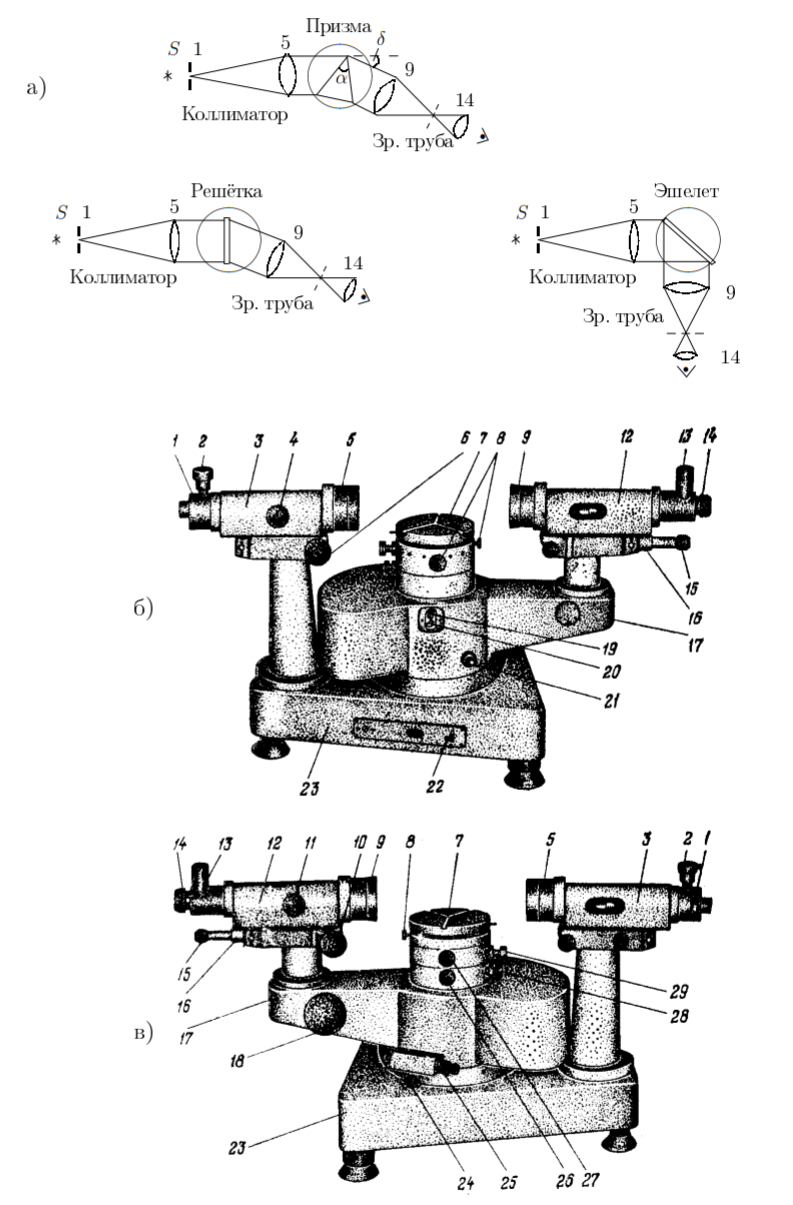
\includegraphics[scale=1]{images/scheme_1.png}
		\caption{Оптическая схема и внешний вид гониометра}
		\label{fig:scheme_1}
	\end{figure}
	
	Оптическая схема гониометра представлена на рис. $\ref{fig:scheme_1}$a. Свет от источника \textit{S} проходит через коллиматор и преобразуется призмой или решеткой в набор параллельных пучков, каждый из который соответсвует определленной длине волны. Параллельные пучки собираются в фокальной плоскости объектива 9 зрительной трубы и рассматриваются глазом через окуляр 14.
	
	Внешний вид гониометра представлен на рис. $\ref{fig:scheme_1}$б и $\ref{fig:scheme_1}$в. Коллиматор 3 столик 7 и алидада 17 со зрительной трубой 12 крепятся на массивном основании 23. На столике 7 размещаются исследуемые объекты. Коллиматор закреплен неподвижно, а столик и алидада с трубой могут вращаться вокруг вертикальной оси.
	
	Ширину коллиматорной цели можно менять при помощи микрометрического винта 2, высоту - при помощи диафрагмы с треугольным вырезом, надетой на щель. Винт 4 служит для перемещения объектива 5 - настройки коллиматора на параллельный пучок.
	
	Зрительная труба 12 состоит из объектива 9 и окуляра 14 с автоколлимационным устройством 13. Фокусировка трубы производится винтом 11. Наклон коллиматора и зрительной трубы к горизонтальной оси изменяется винтами 6 и 10 соответственно.
	
	\begin{wrapfigure}{r}{0.5\linewidth}
		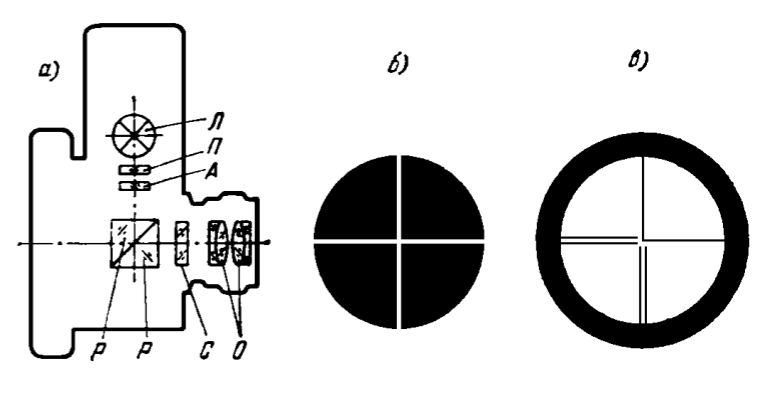
\includegraphics[scale=0.6]{images/scheme_2.png}
		\caption{Автоколлимационное устройство}
		\label{fig:scheme_2}
	\end{wrapfigure}
	
	Схема окуляра О зрительной трубы с автоколлимационным устройством приведена на рис. \ref{fig:scheme_2}а. Свет от лампы Л проходит через защитную стеклянную пластинку П и попадает на автоколлимационную сетку А, содержащую две взаимно перпендикулярные щели. Свет, прошедший через сетку А (светящийся крест - рис. \ref{fig:scheme_2}б), попадает на две прямоугольные призмы P и отражается от гипотенузной грани, на которую нанесён полупрозрачный слой с коэффициентом отражения 50\%.
	
	Обе сетки окуляра, A и C (рис. \ref{fig:scheme_2}а), расположены на строго одинаковых расстояниях от гипотенузных граней призмы P, поэтому их одновременное наблюдение в окуляре возможно только при совпадении фокальных плоскостей объектива и окуляра (труба настроена на бесконечность).
	
	Важнейшим узлом гониометра является устройство, служащее для отсчёта угла поворота зрительной трубы вокруг вертикальной оси, проходящей через центр столика. На этой оси крепится прозрачное кольцо (лимб), расположенное в корпусе прибора. На поверхности лимба нанесена шкала с делениями. Лимб разделён на $3\times 360 = 1080$ делений. Цена деления $20'$, оцифровка деления произведена через $1^{\circ}$. Шкалу лимба можно наблюдать через окуляр отсчётного устройства 16 при включённой подсветке (тумблер 22). Резкость изображения шкалы регулируется вращением оправы окуляра 15.
	
	Оптическая система отсчётного устройства собрана так, что через окуляр можно наблюдать изображения штрихов двух диаметрально противоположных участков лимба, причём одно изображение прямое, а другое обратное (рис. \ref{fig:scheme_3}). Кроме того, оптическа система позволяется перемещать эти изображения друг относительно друга, оставляя в покое как лимб, так и алидаду со зрительной трубой. Это перемещение штрихов измеряется при помощи оптического микрометра. Шкала микрометра рассчитана таким образом, что при перемещении ееё на 600 делений верхнее изображение штрихов лимба смещается относительно нижнего на $10'$. Следовательно, цена деления шкалы микрометра $1''$.
	
	\begin{wrapfigure}{r}{0.6\linewidth}
		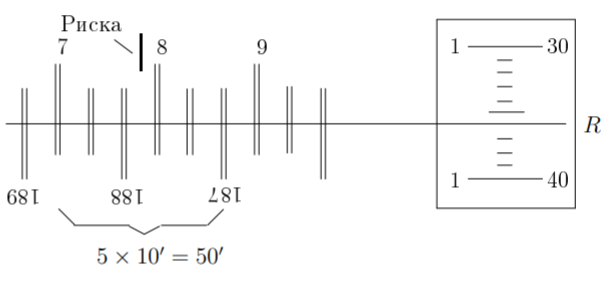
\includegraphics[scale=0.8]{images/scheme_3.png}
		\caption{Поле зрения отсчётного микроскопа ($7^{\circ}51'36''$)}
		\label{fig:scheme_3}
	\end{wrapfigure}
	
	Поле зрения отсчётного микроскопа приведено на рис. \ref{fig:scheme_3}. В левом окне наблюдаются изображения диаметрально противоположных участков лимба и вертикальныз штрих для отсчёта градусов, в правом - деления шкалы оптического микрометра и горизонтальная риска R для отсчёта минут и секунд.
	
	Гониометр требует тщательной юстировки, которая заключается в установке: а) зрительной трубы на бесконечность; б) поверхности столика и оптической оси трубы - перпендикулярно оси вращения прибора; в) коллиматора - на параллельный пучок лучей; г) оптической оси коллиматора - перпендикулярно оси вращения прибора.
	
	\section*{Теоретическая справка}
	
	Угол отклонения материала призмы $n(\lambda )$ удобно определять по углу наименьшего отклонения $\delta (\lambda )$ (рис. \ref{fig:teor_1}). Минимальное отклонение луча, преломлённого призмой, от  направления луча, падающего на призму получается при симметричном ходе луча (в призме луч идёт параллельно основанию). Угол минимального отклонения $\delta$, преломляющий угол $\alpha$ (угол при вершине призмы) и показатель преломления связаны соотношением

	\begin{equation} \label{equation:n(lambda)}
		n(\lambda) = \frac{\sin \frac{\alpha + \delta (\lambda )}{2}}{\sin \frac{\alpha}{2}}
	\end{equation}
	
	\begin{figure}[h!]
		\centering
		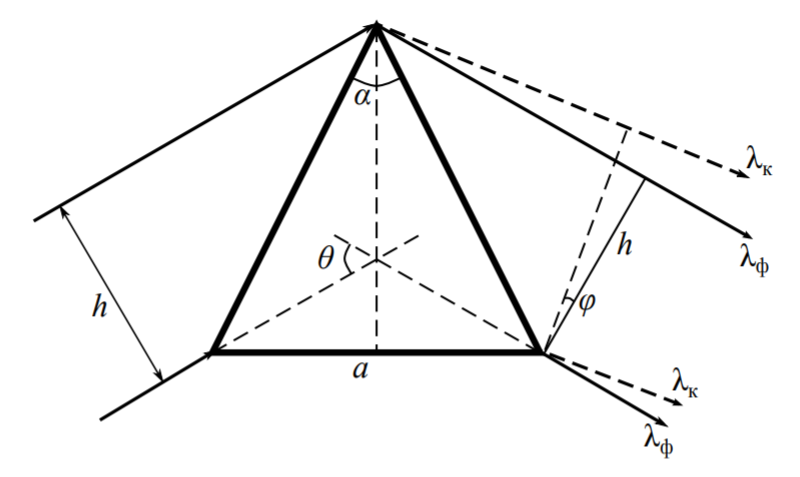
\includegraphics[scale=0.5]{images/teor_1.png}
		\caption{Ход лучей в призме для наименьшего угла отклонения}
		\label{fig:teor_1}
	\end{figure}
	
	\section*{Обработка данных}
	
	Измерим преломляющий угол. Для этого установим трубу перпендикулярно одной из её отражающих граней и сними отсчет по лимбу. Затем повернем алидаду с трубой вокруг преломляющего угла призмы и проведем ту же операцию для другой рабочей грани.
	Рассчитаем преломляющий угол призмы:
	
	\begin{center}
		$\alpha = 59 \degree 12'16''$
	\end{center}

	Вращая столик найдем в окуляре изображение спектра. Для каждого спектра запишем минимальный угол отклонения $\delta$, данные запишем в таблицу \ref{tabel:spectr}.
	
	\begin{table}[h!]
    \centering
    \begin{tabular}{|c|c|c|c|}
    \hline
    $K_1$                 & $K_2$                 & 1                     & 2                     \\ \hline
    $51 \degree 00' 49''$ & $51 \degree 37' 25''$ & $52 \degree 01' 15''$ & $52 \degree 02' 14''$ \\ \hline
    \end{tabular}
    \\[3 mm]
    \begin{tabular}{|c|c|c|c|}
        \hline
        3                     & 4                     & 5                     & 6                      \\ \hline
        $52 \degree 22' 32''$ & $53 \degree 09' 17''$ & $54 \degree 20' 46''$ & $55 \degree 19' 26''$  \\ \hline
    \end{tabular}

    \caption{Наименьший угол отклонения $\delta$ для каждого спектра}
    \label{tabel:spectr}
\end{table}
	
	Используя формулу \eqref{equation:n(lambda)} вычислим показатель преломления для каждого спектра. Результаты запишем в таблицу \ref{table:n}
	
	\begin{table}[h!]
    \centering
    \begin{tabular}{|c|c|c|c|c|c|c|c|c|}
		\hline	
		$\lambda$ нм & 690,7  & 623,4  & 579,1  & 577,0  & 546,1  & 491,6  & 435,8  & 404,7  \\ \hline
		$n$ нм       & 1,6484 & 1,6544 & 1,6583 & 1,6584 & 1,6617 & 1,6693 & 1,6806 & 1,6898 \\ \hline
	\end{tabular}
    \caption{Зависимость показателя преломления от длины волны}
    \label{table:n}
\end{table}
	
	Используя полученные эксперементальные данные построим дисперсионную кривую -- график зависимости $n(\lambda)$.
	
	\begin{figure}
		\centering
		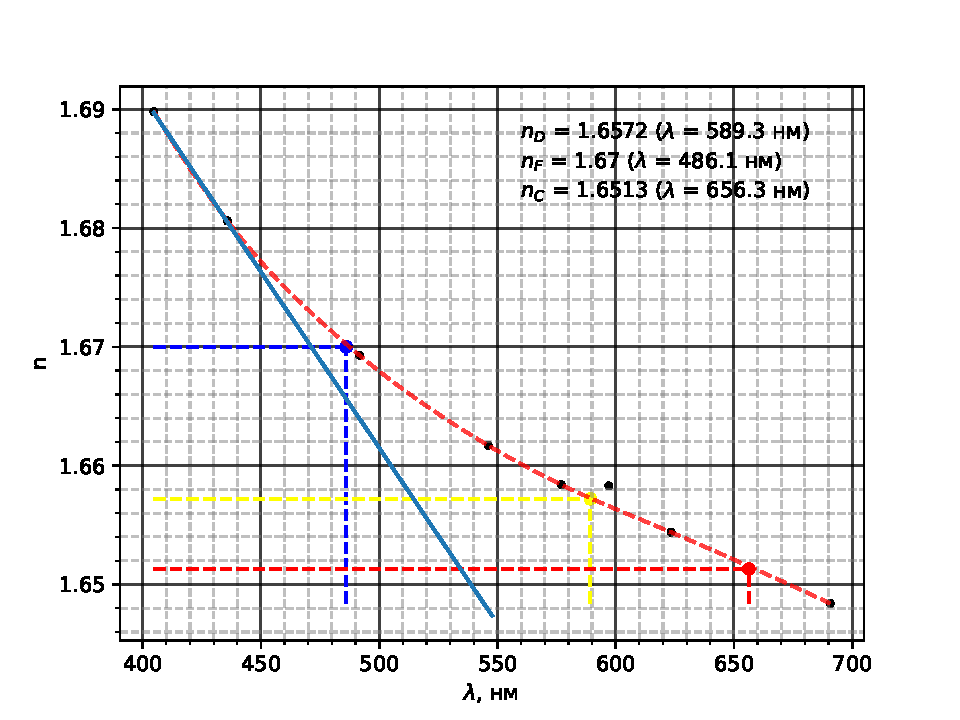
\includegraphics[scale=1]{n_lambda.pdf}
		\caption{Дисперсионная кривая}
		\label{figure:n_lambda}
	\end{figure}

	По графику определим величины:
	
	\begin{center}
		$n_D = 1.6572 ~ \pm ~ 0.0001$ \\
		$n_F = 1.6700 ~ \pm ~ 0.0001$ \\
		$n_C = 1.6513 ~ \pm ~ 0.0001$ \\
	\end{center}

	Вычислим среднюю дисперсию стекла по формуле:
	
	\begin{equation}
		D = n_F - n_C = 0.0187 ~ \pm ~ 0.0001
	\end{equation}
	
	Вычислим число Аббе по формуле:
	
	\begin{equation}
		\nu = \frac{n_D - 1}{n_D - n_C} = 35.13 ~ \pm ~ 0.0037
	\end{equation}
	
	Для оценки разрешающей способности призмы измерили угловую ширину жёлтых линий дублета, предварительно установив минимально возможную ширину входной щели:
	\begin{center}
		\begin{tikzpicture}
		\fill[fill=black!20] (0,0) -- (-1.5,0) -- (-1.5,2) -- (0,2);
		\fill[fill=black!20] (1.2,0) -- (0.7,0) -- (0.7,2) -- (1.2,2);
		\fill[fill=black!20] (1.8,0) -- (3.3,0) -- (3.3,2) -- (1.8,2);
		\draw[dashed] (0,0) -- (0,2);
		\draw[dashed] (0.7,0) -- (0.7,2);
		\draw[dashed] (1.2,0) -- (1.2,2);
		\draw[dashed] (1.8,0) -- (1.8,2);
		\fill (0,1) circle (0.05) node[left] {$x_0$};
		\fill (0.7,1) circle (0.05) node[above left] {$x_1$};
		\fill (1.2,1) circle (0.05) node[above right] {$x_2$};
		\fill (1.8,1) circle (0.05) node[right] {$x_3$};
		\end{tikzpicture}
		\\
		\vspace{0.4cm}
		\begin{tabular}{|c|c|c|c|}
			\hline
			$x_0$ & $x_1$ & $x_2$ & $x_3$ \\ \hline
			$7'15''$  & $6'41''$ & $5'54''$ & $5'24''$ \\ \hline
		\end{tabular}
	\end{center}
	Измерили линейкой длину $b=7{,}4\pm0{,}1$ см основания призмы.
	
	По наклону дисперсионной кривой $\frac{d n}{d \lambda}$ определим максимальную разрешающую способность призмы
	
	\begin{equation}
		R = b \frac{d n}{d \lambda} = 21904 ~ \pm ~ 418
	\end{equation}
	
	где $b$ -- размер основания призмы, если вся рабочая грань призмы освещена параллельным пучком. $\frac{d n}{d \lambda} = (29.6 ~ \pm ~ 0.4) \cdot 10^4 ~ m^{-1}$
	
	Экспериментальная величина по измерениям желтого дублета:
	\[ R > \frac{\lambda}{\delta \lambda} \approx 255 \] 
	
	Оценим, при каком размере решетки плотностью, имеющей 100 шт/мм, она обладает такой же разрешающей способностью в первом порядке, как призма с основанием $b = 5$ см.
	
	\[ x \cdot 100 = R = b \frac{d n}{d \lambda} \Rightarrow x = 148 ~ \text{мм} \] 
	
\end{document}